\documentclass[11pt]{article}
\newcommand{\beq}{\begin{equation}}
\newcommand{\eeq}{\end{equation}}
\setlength{\parindent}{0pt}
\usepackage{graphicx}
\usepackage{float}
\graphicspath{ {images/} }
\usepackage{url}
\usepackage{listings}
\title{TTM4110 Simulation Lab Report}
\date{{\today}}
\begin{document}
\pagestyle{plain}

\maketitle

\section{Report}

\subsection{Introduction}

In this lab, we will be simulating a smart grid system. The lab is divided into two parts, part one focuses mainly on performance, while part two focuses on availability and dependability. These aspects are important to consider when building a complex system such as a smart grid. Simulation can be an excellent tool in estimating unknown parameters given a set of known or otherwise estimated parameters.

Both tasks will be solved by discrete event simulation using SIMULA with the DEMOS-library.

The objective in task one is to estimate the delay, depending on how many devices are connected, and how many servers the ELHUB has to handle the load.

The objective in task two is to estimate the downtime of the system.


\newpage
\subsection{Answer to questions}

\subsubsection{Task 1}

1) The system state is defined in the course book as the set of variables describing the system at time t. The system state thus consists of the following variables:\\
- The number of packets traversing the system\\
- The individual timestamps and delay times of the packets traversing the system\\
- The queues at the controller and servers\\
- The probability of packet loss (between the smart meters and the base stations).\\

The events in this system are the transmission of packets between nodes in the network - from the smart meters to the base stations, from the base stations through the network to the controller and from the controller to one of the servers.\\

\newpage

2) 

\begin{figure}[H]
	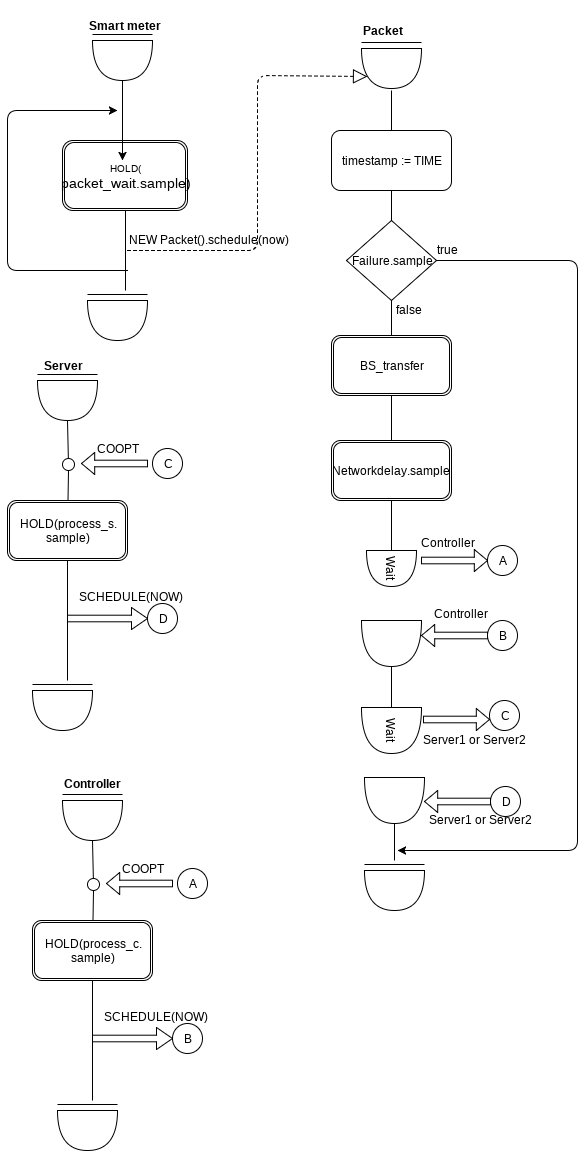
\includegraphics[width=\textwidth,height=0.9\textheight,keepaspectratio]{activiy_diagram1.png}
	\centering
\end{figure}

\newpage


3)\\
See the appendix for the complete code. I have chosen not to include the base stations or the network as entities in my models because they are constant, and do not change over time, as opposed to packets (timestamp) and the controller and servers (queues). The intensity has been chosen in an arbitrary way, using the following assumptions:\\
- A smart meter sends out updates two times per hour.\\
- Updates consists of 100kB, and each packet carries (on average) 1000 bytes of data.\\\\
This gives an intensity $\lambda$ of $\frac{200kB}{1000B \cdot 60 \cdot 60} = 0.055555 \approx 0.06$ packets per second.
Given that this is the result of a Poisson process, the time between packets is negatively exponentially distributed with parameter $\lambda$.

It is worth noting that all time is calculated in seconds in this implementation of the simulation.

Simulating with one smart meter, 50 base stations and two servers gives the following result.

\begin{figure}[H]
	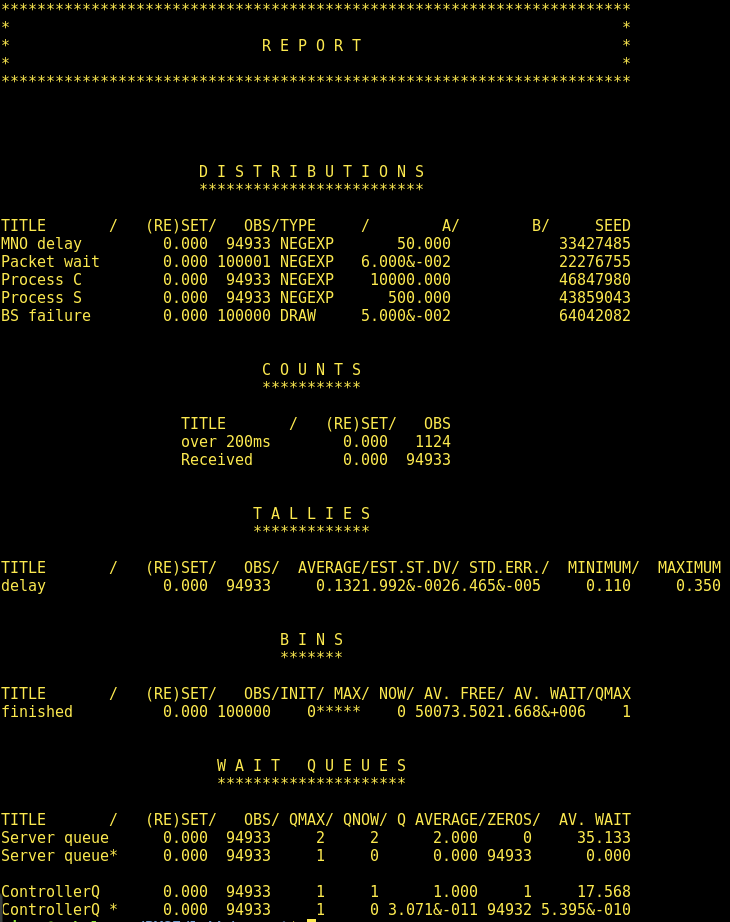
\includegraphics[width=\textwidth]{demos_1.png}
	\centering
\end{figure}

We see from the image that $P(T < 200) \approx 1124 / 10000 = 0.1124$


4)\\ It appears that when we increase the numbers of smart meters, the delay increases. This makes sense, as more smart meters means more packets, meaning longer queue-times. The delay time seems to be about equal when looking at small numbers of smart meters, however when reaching larger numbers, the delay time increases at a slower pace with more servers than with fewer. This is reasonable, as queues will fill up faster when fewer servers are handling packets.

Note that it appears that the packet loss increase, but this is probably not true. What is happening is that packets dropped are recorded earlier, while more succesful packets are stuck in queues. This is simply a side effect of having a set number of packets, and recording lost packets the instant they are lost.

Summarized:

\begin{lstlisting}
N_s = 2:

N_sm = 1000:
TITLE OBS/  AVERAGE/EST.ST.DV/ STD.ERR./  MINIMUM/  MAXIMUM
delay 94932   0.1321.991&-0026.462&-005     0.110     0.350

N_sm = 10000:
TITLE OBS/  AVERAGE/EST.ST.DV/ STD.ERR./  MINIMUM/  MAXIMUM
delay 94929   0.1332.000&-0026.490&-005     0.110     0.349

N_sm = 100000:
TITLE OBS/  AVERAGE/EST.ST.DV/ STD.ERR./  MINIMUM/  MAXIMUM
delay 77136   31.538    18.2076.555&-002     0.112    63.272


N_s = 4:

N_sm = 1000:
TITLE OBS/  AVERAGE/EST.ST.DV/ STD.ERR./  MINIMUM/  MAXIMUM
delay 94932   0.1321.991&-0026.461&-005     0.110     0.350

N_sm = 10000:
TITLE OBS/  AVERAGE/EST.ST.DV/ STD.ERR./  MINIMUM/  MAXIMUM
delay 94929   0.1321.990&-0026.460&-005     0.110     0.348

N_sm = 100000:
TITLE OBS/ AVERAGE/EST.ST.DV/ STD.ERR./  MINIMUM/  MAXIMUM
delay 86986  14.037     8.0822.740&-002     0.112    28.215

\end{lstlisting}

Put into a graph, red being for $N_s = 2$, blue being $N_s = 4$.

\begin{figure}[H]
\begin{center}
	\makebox[\textwidth]{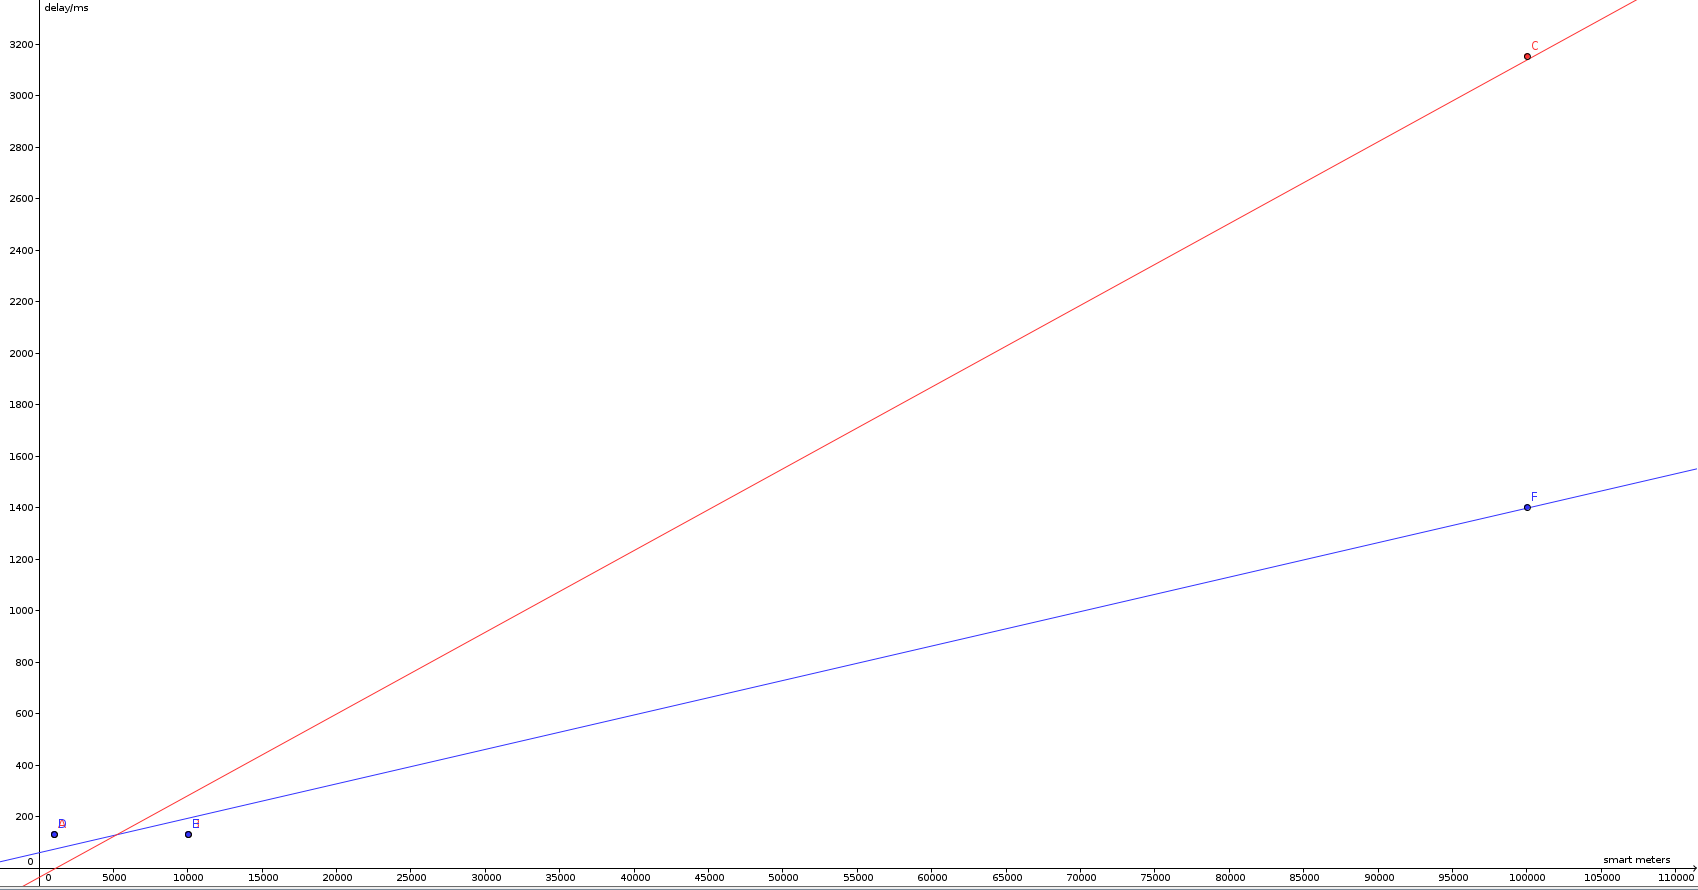
\includegraphics[width=\paperwidth]{geogebrabilde.png}}
\end{center}
\end{figure}

The program version with a logging function is attached in the appendix.

5)

If a packet is lost, it is not taken into account when calculating the delay, nor is it taken into account when plotting the CDF for the delay as the delay of a dropped packet is undefined.
Parameters set for the generation of this data: $N_s = 2, N_sm = 10000$.
$$94929\ packets\ sent,\ 5071\ packets\ lost\ \Rightarrow$$ $$\ P(packet\ lost)\ = 0.053418870 \approx 5.342\%$$

This is somewhat higher than what should be the case - 5\%. This could be due to a multitude of reasons, among them the fact that lost packets are recorded at once, while packets that are not lost are recorded when they arrive at a server. This would mean that several successful packets are still in the pipeline when the simulation terminates after 10 000 total packets (lost and received). Ergo is this a side effect of the way the simulation is implemented. If packet loss was what we wished to estimate, the simulation would have to have been done differently.


CDF for end-to-end packet delay on the same data:

\begin{figure}[H]
	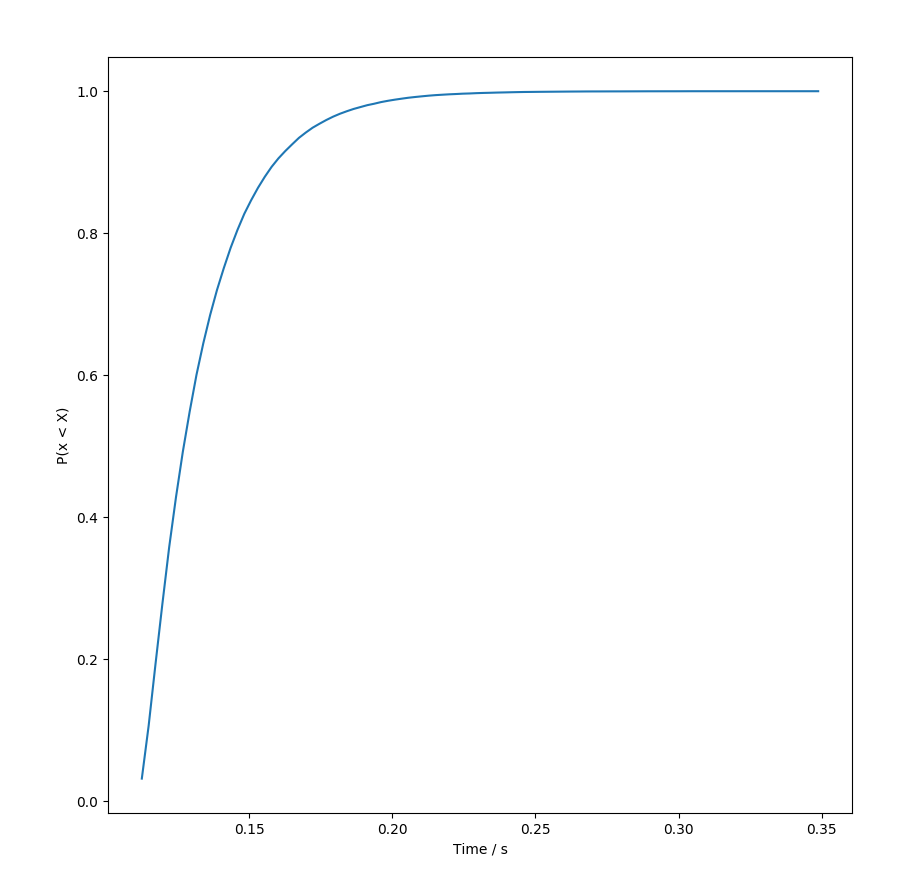
\includegraphics[width=\textwidth]{cdf_plot.png}
	\centering
\end{figure}

No packets use less time than the transfer time between a smart meter and a base station (constant), and no packets use longer time than 350 ms in this case, using the specific constants above.\\


The python-script used to generate the plot can be found in the appendix. The data is generated using the code from task 1-3, also found in the appendix.


\subsubsection{Task 2}

1) The system states are now:\\
- One or more server(s) up, controller up\\
- No servers up, controller up\\
- One or more server(s) up, controller down\\
- No servers up, controller down\\

The events being a server going up/down and the controller going up/down.
The ELHUB is unavailable when the controller is down, or when no servers are up, or both.\\

2) \\
\begin{figure}[H]
	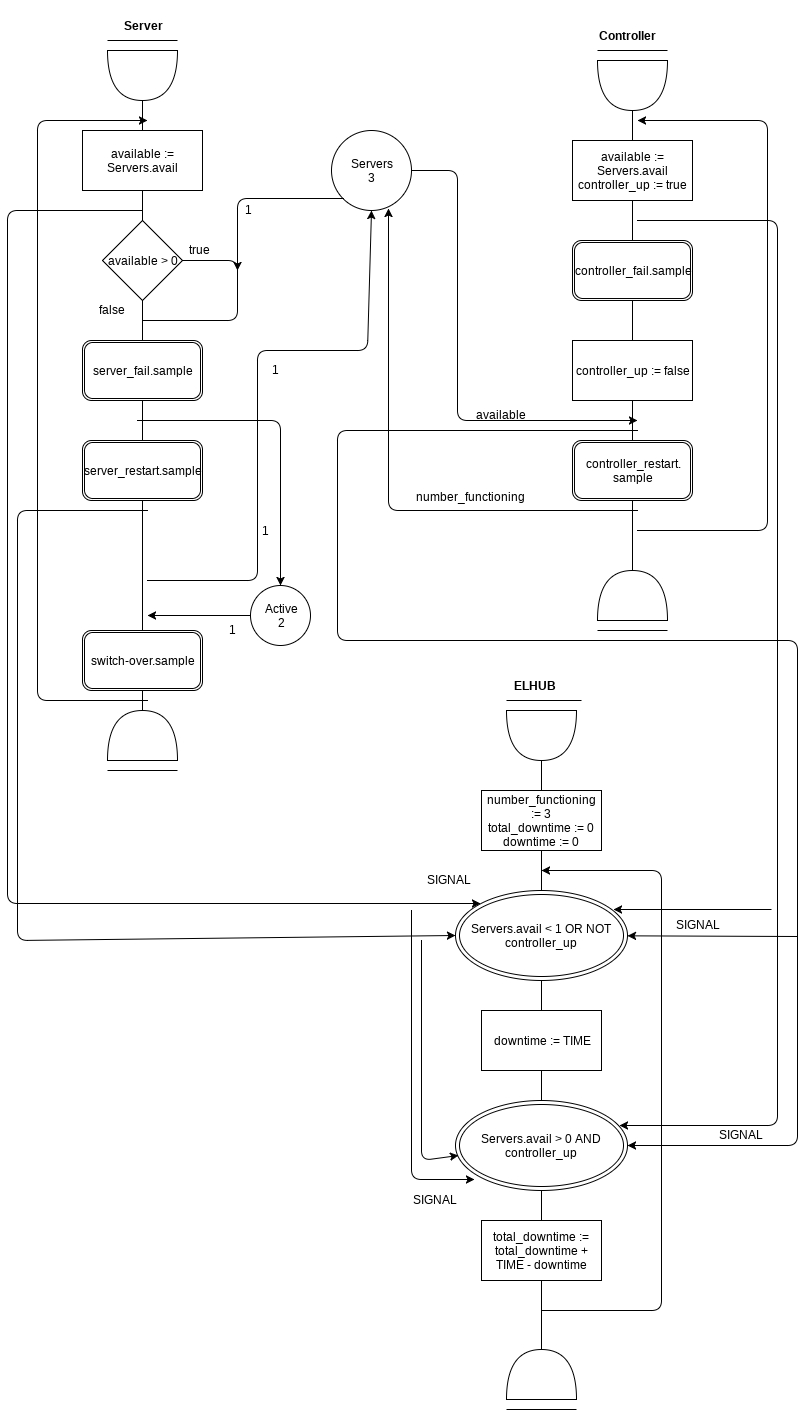
\includegraphics[width=\textwidth]{activity_diagram2.png}
	\centering
\end{figure}

See the appendix for the code.

The implementation uses the resource-class to keep track of the servers, both available and passive. A server has two states; passive and active. I have made the following assumptions in this task:\\
- When a server restarts, it is fixed, and after a restart it is instantly passive.\\
- A server cannot fail while in passive mode\\

I think these are reasonable assumptions - servers may fail for no "reason" at all, but it is much more likely to fail when stressed. Therefore I assume the probability that an idle server failing is trivial. A server going into passive mode after a restart, and then into active mode if needed, and after a switch-over time is also a fair assumption.\\

The hub entity tracks when the conditions for up and down are met, and records the time the ELHUB is down. This is done using a conditional queue, which the server and controller entities signal when a change happens.

Note that in passive mode, a server awaits an active-token before it holds for a switch-over time, and then goes into the active state.\\

3)\\
Result of a run of the simulation with sim\_time set to 1 million, and the parameters set to the first set:

\begin{figure}[H]
	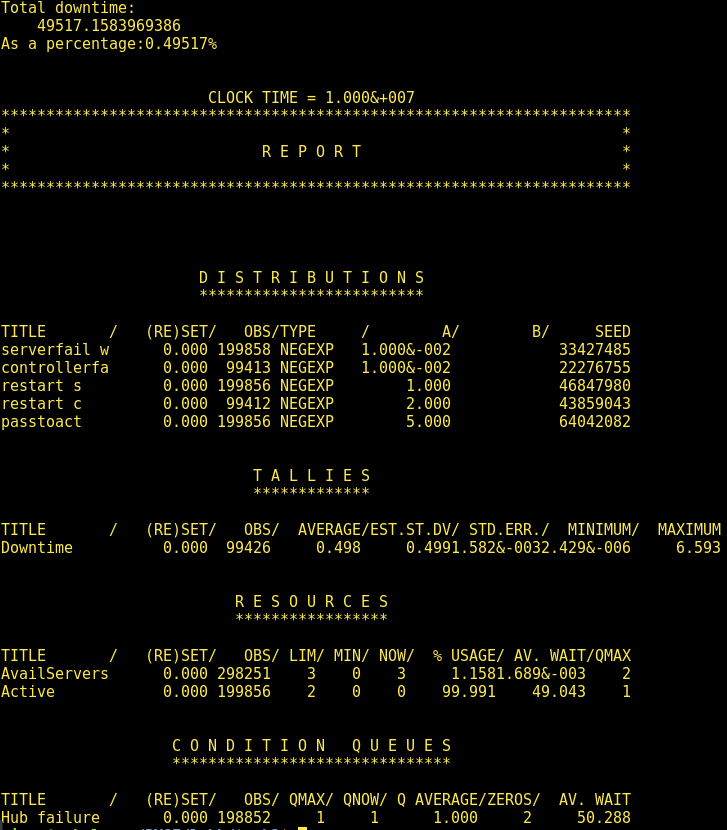
\includegraphics[width=\textwidth]{demos_2-2.png}
	\centering
\end{figure}

Below is the result of a run of the simulation with sim\_time set to 1 million, and using the alternative values for $\lambda_{fc}$ and $\mu_{sw}$.

\begin{figure}[H]
	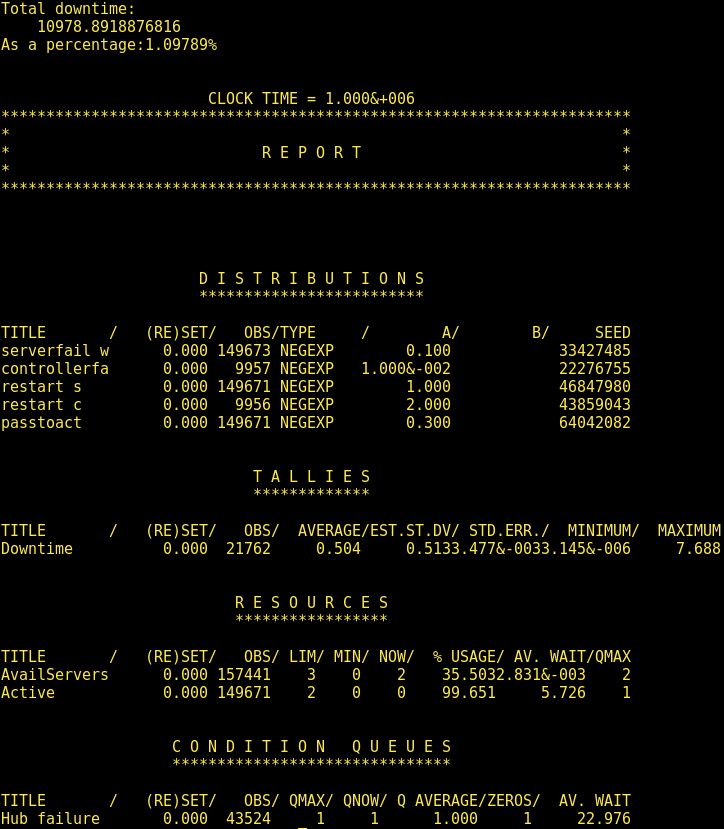
\includegraphics[width=\textwidth]{demos_2-2_alt.png}
	\centering
\end{figure}

4)\\ I have solved this task wile assuming the switch-over time is non-zero. The resulting downtimes, given both given sets of parameters gave the results that are attached for the previous answer.

To make this easily accessible my downtime results can be found below as well. Keep in mind this is with a simulation time of 1 million.

$$Simulated: \mu_{sw} = 5, \lambda_{fc} = 0.01 \Rightarrow U_{hub} = 0.50769\%$$

$$Simulated: \mu_{sw} = 0.3, \lambda_{fc} = 0.1 \Rightarrow U_{hub} = 1.09789\%$$

Using the analytic expression given for $U_s$ when the switch-over time is non-zero gives:

$$U_s \approx \frac{\lambda_{fs}^3(\lambda_{fs}(4\mu_{rs}^2 + 9\mu_{rs}\mu_{sw} + 3\mu_{sw}^3))}{3\mu_{rs}^2(\mu_{rs}+\mu_{sw})(\lambda_{fs}(8\mu_{rs} + 3\mu_{sw}) + \mu_{rs}(2\mu_{rs}+\mu_{sw})} $$

$$U_{hub} = U_s + U_c - U_s \cdot U_c$$

Inserting $U_s$ and $U_c$ into the equation for $U_{hub}$ yields respectively:

$$Analytically: \mu_{sw} = 5, \lambda_{fc} = 0.01 \Rightarrow U_{hub} = 0.49807\%$$

$$Analytically: \mu_{sw} = 0.3, \lambda_{fc} = 0.1 \Rightarrow U_{hub} = 1.03314\%$$

The simulated downtime is not equal to the analytical downtime, but it is not far off. This may be due to an error in my simulation, but I think it more likely that it is caused by the random behaviour of stochastic processes. If the simulation time tends towards infinity, the simulated downtime should tend towards the analytical downtime.




\newpage
\subsection{Summary}

In this lab, we have looked at the performance and dependability of a smart grid. We have simulated the delay of packets traversing the system, and the uptime of parts of the system.\\

After this lab, it has become more apparent how useful simulation can be, and how straight forward and close to the analytical results in can be, as opposed to dealing with difficult and long analytical expressions.

\subsubsection{Task 1}
Simulating the delay and packet loss as packets traverse the system from smart meters all the way to the ELHUB-servers showed how useful simulation can be while looking at delay of packets through complex systems with multiple moving parts. I think the results achieved in this task are reasonable given the given constants. We saw here that when there are few smart meters, the delay is low, and mostly dictated by the stochastic processes - varying from 110 ms to 350 ms. When we increased the number of smart meters, and thereby the number of packets traversing the system at the same time, the delay went up - in some cases drastically. Here, the stochastic processes are no longer the biggest deciding factor - now the queues cause packets to mass up, waiting to be handled by the controller and the servers. Increasing the number of servers handling the load helped decrease the growth rate of delay as a function of number of smart meters, but the increase from two servers to four was not enough to keep packets at a reasonable level of delay.

It should be apparent, at least after this simulation, that two or four servers with the given processing time cannot provide enough capacity for 100 000 or 1 000 000 smart meters. This is not really realistic either - in a real world scenario it is likely that the ELHUB-company would use more servers, and probably servers with shorter processing times.

\subsubsection{Task 2}

The downtime of a critical system such as the ELHUB is an important factor for the responsible business to think of when planning around it. It has therefore been interesting to simulate this in this lab.

The results in my simulation did not completely match the analytical results. Nonetheless my results were close to the analytic result, and while it is possible that I have made mistakes in my code, I think the more likely explanation, as outlined earlier, is the fact that downtime is a result of stochastic processes. Especially considering how close my results are using both sets of given variables.

The code was difficult to write though, so one or several mistakes are probable.
\\
\\

All in all, this has been an interesting lab, teaching a lot of useful concepts in a trial-by-fire way. 

\newpage
\section*{Appendix}

\subsubsection{Code from task 1-3}

\begin{lstlisting}

BEGIN
EXTERNAL CLASS demos = "../demos/demos.atr";
demos BEGIN

REAL Tw, Tn, Tc, Ts, p_r, intensity;
INTEGER num_BS, sim_n, num_s, num_meters, i, j, meters_per_bs, packet_n;
REF(Bin) finished_packets;
REF(RDist) MNO_delay, process_c, process_s, packet_wait;
REF(BDist) BS_failure;
REF(Tally) emp_delay;
REF(WaitQ) serverq, controllerq;
REF(Count) over, packets_recv;

ENTITY CLASS SM;
BEGIN
INTEGER i;

LOOP:
hold(packet_wait.sample);
NEW Packet(edit("pakke",i)).schedule(now);
i := i + 1;
packet_n := packet_n + 1;
REPEAT;
END;



ENTITY CLASS Packet;
BEGIN
LONG REAL ts;
ts := time;
if BS_failure.sample then BEGIN
finished_packets.give(1);
!outInt(packet_n, 8);
!outText(",");
!outInt(0,1);
!outimage;
END
ELSE BEGIN
hold(Tw);
hold(MNO_delay.sample);

controllerq.wait; 
serverq.wait;

emp_delay.update(time - ts);

if (time - ts) > 0.200 then over.update(1);
finished_packets.give(1);
packets_recv.update(1);

! Uncomment to get a trace of packets;
!outInt(packet_n, 8);
!outText(",");
!outfix(time - ts, 7, 12);
!outimage;
END;
END;

ENTITY CLASS Controller(waitq_);
REF(WaitQ) waitq_;
BEGIN
REF(Packet) pakka;

LOOP:
pakka :- waitq_.coopt;
hold(process_c.sample);
pakka.schedule(now);        
REPEAT;
END;

ENTITY CLASS Server(waitq_);
REF(WaitQ) waitq_;
BEGIN

REF(Packet) pakka;

LOOP:
pakka :- waitq_.coopt;
hold(process_s.sample);
pakka.schedule(now);
REPEAT;   
END;


! Variable numbers;
Tw := 110 / 1000;
Tn := 20 / 1000;
Tc := 0.1 / 1000;
Ts := 2 / 1000;
p_r := 0.95;
num_BS := 50;
num_s := 2;
sim_n := 100000;
num_meters := 10000;
packet_n := 0;
meters_per_bs := num_meters / num_BS;
intensity := 0.06;

! Distributions;
MNO_delay :- NEW NegExp("MNO delay", 1/Tn);
packet_wait :- NEW NegExp("Packet wait", intensity);
process_c :- NEW NegExp("Process C", 1/Tc);
process_s :- NEW NegExp("Process S", 1/Ts);
BS_failure :- NEW Draw("BS failure", 1 - p_r);

! Variable classes;
emp_delay :- NEW Tally("delay");

finished_packets :- NEW Bin("finished", 0);
serverq :- NEW WaitQ("Server queue"); 
controllerq :- NEW WaitQ("ControllerQ");

! Counts ;
over :- NEW Count("over 200ms");
packets_recv :- NEW Count("Received");

! Instantiate classes my dudes;
NEW Controller("C", controllerq).schedule(0.0);

for i:=1 step 1 until num_s do
NEW Server(edit("Server",i), serverq).schedule(0.0);

for i:=1 step 1 until num_meters do
NEW SM(edit("SM",i)).schedule(0.0);

finished_packets.take(sim_n);

END;
END;


\end{lstlisting}

\subsubsection{Python code used to generate CDF-graph}
Note: the file results.csv, generated by the above code, has to be in the same folder as the script, in order to run.
\begin{lstlisting}
#!/usr/bin/python2.7
import numpy as np
import matplotlib.pyplot as plt

with open('results.csv','r') as f:
	lines = [x.split(',') for x in f.readlines()]

data = []
for line in lines:
	tmp = [x.strip() for x in line]
	data.append(tmp)
raw = []
for line in data:
	if line[-1] != 0 and line[-1] != '0':
		raw.append(float(line[-1]))

print "[*] Estimating probability of packetloss.."

lost = 0
for k in data:
	if k[1]=='0': lost+=1

print "{} packets sent, {} packets lost => P(packet lost) = {}".format(len(raw), lost, float(lost)/len(raw))

arr = np.array(raw)

h, X1 = np.histogram(arr, bins=100, normed=True)
dx = X1[1] - X1[0]
F1 = np.cumsum(h) * dx

plt.plot(X1[1:], F1)
plt.xlabel("Time / s")
plt.ylabel("P(x < X)")

plt.show()
\end{lstlisting}

\subsubsection{Code from task 2-2 and 2-3}


\begin{lstlisting}
BEGIN
EXTERNAL CLASS DEMOS = "../demos/demos.atr";
DEMOS BEGIN

REAL tot_downtime, server_fail_intensity, controller_fail_intensity, restart_s_mean, restart_c_mean, pass_to_act_mean, sim_time;
INTEGER num_server;
REF(RDIST) server_fail_wait, controller_fail_wait, restart_s, restart_c, pass_to_act;
REF(RES) available_servers, active_;
BOOLEAN controller_up;
REF(CONDQ) hub_failure;
REF(TALLY) downtime_;

ENTITY CLASS SERVER(init_);
BOOLEAN init_;
BEGIN
INTEGER available;

if not init_ THEN goto passive;
active_.acquire(1);

active:
available := available_servers.avail;

if available > 0 THEN
BEGIN
HOLD(server_fail_wait.sample);
available_servers.acquire(1);
hub_failure.signal;

active_.release(1);

HOLD(restart_s.sample);

if (controller_up) THEN
BEGIN
available_servers.release(1);
hub_failure.signal;
END;
END
ELSE
BEGIN

HOLD(server_fail_wait.sample);
active_.release(1); 

HOLD(restart_s.sample);
END;

passive:
active_.acquire(1);
HOLD(pass_to_act.sample);
goto active;
END;

ENTITY CLASS CONTROLLER;
BEGIN
INTEGER available;

LOOP:

HOLD(controller_fail_wait.sample);
controller_up := false;

available := available_servers.avail;

if available > 0 THEN 
BEGIN
available_servers.acquire(available);
END;
hub_failure.signal;

HOLD(restart_c.sample);

if active_.avail < 2 THEN available_servers.release(2 - active_.avail);

controller_up := true;
hub_failure.signal;
REPEAT;
END;

! ELHUB-class. Keeps track of downtime using a conditional queue;
ENTITY CLASS HUB;
BEGIN
INTEGER available;
LONG REAL downtime;

! The Hub is down when 0 servers are available, or the controller is down;
LOOP:
hub_failure.waituntil(available_servers.avail < 1 or not controller_up);
downtime := time;
hub_failure.waituntil(available_servers.avail > 0 and controller_up);
downtime := time - downtime;
tot_downtime := tot_downtime + downtime;
downtime_.update(downtime);
REPEAT;
END;

! System variables;
server_fail_intensity := 0.1;
controller_fail_intensity := 0.01;
restart_s_mean := 1;
restart_c_mean := 2;
pass_to_act_mean := 0.3;
controller_up := true;
num_server := 3;
tot_downtime := 0;

! DEMOS-objects and distributions;        
downtime_ :- NEW TALLY("Downtime");
hub_failure :- NEW CONDQ("Hub failure");
available_servers :- NEW RES("AvailServers", num_server);
active_ :- NEW RES("Active", 2);


server_fail_wait :- NEW NegExp("serverfail wait", server_fail_intensity);
controller_fail_wait :- NEW NegExp("controllerfail wait", controller_fail_intensity);
restart_s :- NEW NegExp("restart s", restart_s_mean);
restart_c :- NEW NegExp("restart c", restart_c_mean);
pass_to_act :- NEW NegExp("passtoact", pass_to_act_mean);

! Initialise objects;
NEW HUB("Hub").schedule(0.0);
NEW CONTROLLER("C1").schedule(0.0);
NEW SERVER("S1", true).schedule(0.0);
NEW SERVER("S2", true).schedule(0.0);
NEW SERVER("S3", false).schedule(0.0);

! Arbitrarily chosen number for keeping simulation going;
sim_time := 10000000;
HOLD(sim_time);

! Output recorded downtime;
outText("Total downtime:");
outimage;
outFix(tot_downtime, 10, 20);
outimage;
outText("As a percentage:");
tot_downtime := tot_downtime / sim_time * 100;
outFix(tot_downtime, 5, 7);
outText("%");
outimage;

END;
END;


\end{lstlisting}


\end{document}